\documentclass[a4paper, oneside, 10pt]{article}

\usepackage[american]{babel}

\usepackage{ifthen}
\usepackage{tabularx}
\usepackage{tikz}
\usepackage{marginnote}
\usepackage{csquotes}

\usepackage{amsmath}
\usepackage{mathtools}

\usepackage[a4paper]{geometry}
\geometry{left=4.5cm, right=3cm, top=3cm, bottom=3.5cm,
          heightrounded, headheight=12.1pt,
          marginparwidth=3cm, marginparsep=0.75cm, footskip=2cm}
\reversemarginpar

\usepackage[light,condensed]{roboto}                      % Sans Serif
\usepackage[default,light,semibold,tabular]{sourceserifpro} % Roman
\usepackage[varqu]{zi4}                                    % Monotype
\makeatletter
\def\bfseries@sf{b}
\makeatother
\newcommand{\RobotoCon}{\sffamily}
\newcommand{\Roboto}{\sffamily}
\newcommand{\SpaceRoboto}{\sffamily}

\usepackage{microtype}

\usepackage{xcolor}
\definecolor{darkred}{HTML}{CF232B}
\definecolor{darkblue}{HTML}{2B23CF}
\definecolor{darkgray}{HTML}{555555}
\definecolor{lightgray}{HTML}{cccccc}
\colorlet{citecolor}{black}
\colorlet{linkcolor}{darkgray}
\colorlet{urlcolor}{darkgray}

\usepackage{titlesec}

\titleformat{\section}{\Large\sffamily\bfseries}
            {\llap{{\textcolor{lightgray}{\normalfont\sffamily\thesection}}\hskip 0.5em}}{0em}{}
\titleformat{\subsection}{\large\sffamily\bfseries}
     {\llap{{\textcolor{lightgray}{\normalfont\sffamily\thesubsection}}\hskip 0.5em}}{0em}{}

\titleformat{\subsubsection}[runin]
            {\normalfont\sffamily\bfseries}{}{0em}{}[\mbox{ --- }]
\titlespacing{\subsubsection}
             {0pt}                        % left
             {3.25ex plus 1ex minus .2ex} % before
             {0pt}                        % after

\usepackage[labelsep=period]{caption}
\renewcommand{\captionfont}{\small}
\renewcommand{\captionlabelfont}{\small\sffamily\bfseries}

\usepackage[pdfusetitle,
            bookmarks=true,
            breaklinks=true,
            pdfborder={0 0 0},
            citecolor=citecolor,
            linkcolor=linkcolor,
            urlcolor=urlcolor,
            colorlinks=true,
            linktocpage=false,
            hyperindex=true,
            colorlinks=true,
            linktocpage=false,
            linkbordercolor=white]{hyperref}
\hypersetup{linkcolor=black,urlcolor=darkgray}
\urlstyle{sf}

\usepackage{listings}
\lstset{%
  basicstyle=\ttfamily\small,
  keywordstyle=\color{black},
  commentstyle=\color{gray},
  stringstyle=\color{black},
  backgroundcolor=\color{white},
  numbers=none,
  numberstyle=\ttfamily,
  stepnumber=2,
  showspaces=false,
  showstringspaces=false,
  showtabs=false,
  frame=none,
  framerule=0.5pt,
  tabsize=2,
  rulesep=5em,
  captionpos=b,
  breaklines=true,
  breakatwhitespace=false,
  framexleftmargin=0em,
  xleftmargin=0em,
  framexrightmargin=0em,
  xrightmargin=0em,
  aboveskip=0.5em,
  belowskip=0.5em,
}

\setlength\parindent{0pt}

\usepackage{enumitem}

\renewcommand*{\marginfont}{\scriptsize\sffamily}

\usepackage{authblk,etoolbox}
\makeatletter
\patchcmd{\@maketitle}{center}{flushleft}{}{}
\patchcmd{\@maketitle}{center}{flushleft}{}{}
\patchcmd{\@maketitle}{\LARGE}{\LARGE\sffamily\bfseries\vspace{-2.em}}{}{}
\def\maketitle{{%
  \renewenvironment{tabular}[2][]
    {\begin{flushleft}}
    {\end{flushleft}}
  \AB@maketitle}}
\makeatother
\setlength{\affilsep}{0.25em}
\renewcommand\Affilfont{\normalfont\sffamily\footnotesize}
\renewcommand\Authfont{\sffamily\bfseries\small}
\makeatletter
\renewcommand\AB@affilsepx{ -- \protect\Affilfont}
\makeatother

\usepackage[many]{tcolorbox}
\newtcbox{\iconbox}[1][]{%
  enhanced,nobeforeafter,tcbox raise base,
  boxrule=0.4pt, top=0pt, bottom=-1pt,
  right=.1pt, left=.1pt, arc=1pt, boxsep=1pt,
  fontupper={\tiny \sffamily}, before upper={\vphantom{dlg}},
  colframe=white, colback=black!10!white, coltext=black}
\newcommand{\orcid}[1]{\href{https://orcid.org/#1}{\iconbox{ID}}}
\newcommand{\doi}[1]{\href{http://oadoi.org/#1}{#1}}
\newcommand{\github}[1]{\href{https://github.com/#1}{github.com/#1}}

\newcommand{\ExternalLink}{%
    \tikz[x=1.2ex, y=1.2ex, baseline=-0.05ex]{%
        \begin{scope}[x=1ex, y=1ex]
            \clip (-0.1,-0.1)
                --++ (-0, 1.2)
                --++ (0.6, 0)
                --++ (0, -0.6)
                --++ (0.6, 0)
                --++ (0, -1);
            \path[draw,
                line width = 0.5,
                rounded corners=0.5]
                (0,0) rectangle (1,1);
        \end{scope}
        \path[draw, line width = 0.5] (0.5, 0.5)
            -- (1, 1);
        \path[draw, line width = 0.5] (0.6, 1)
            -- (1, 1) -- (1, 0.6);
        }
    }

\def \codeURL{https://github.com/AngadKumar16/ReScience-C}
\def \codeDOI{}
\def \codeSWH{}
\def \dataURL{}
\def \dataDOI{}
\def \editorNAME{}
\def \editorORCID{}
\def \reviewerINAME{}
\def \reviewerIORCID{}
\def \reviewerIINAME{}
\def \reviewerIIORCID{}
\def \dateRECEIVED{}
\def \dateACCEPTED{}
\def \datePUBLISHED{}
\def \articleTITLE{[Re] Reliable evaluation of the quantal determinants of synaptic efficacy using Bayesian analysis}
\def \articleTYPE{Replication}
\def \articleDOMAIN{Computational Neuroscience}
\def \articleBIBLIOGRAPHY{bibliography.bib}
\def \articleYEAR{2026}
\def \reviewURL{}
\def \articleABSTRACT{Bhumbra and Beato (2013) introduced Bayesian Quantal Analysis (BQA), which infers the quantal parameters of synaptic transmission from recorded response amplitudes by evaluating the posterior on a fixed grid. We reimplemented BQA just using their paper, without reading or implementing the authors' code. The likelihood and grid inference were reproduced. We also ran simulation-based calibration, which the original paper did not run. This shows unbiased point estimates and calibrated total-response, variability and site-count marginals. The quantal-size interval is conservative, covering 94.5 percent at a nominal 90 percent, because of the sum over candidate site counts. A first version of this analysis reported the opposite, caused by an off-by-half-cell error in our own rank statistic, which we write about. We also map identifiability across the release-probability contrast, compare BQA with multiple-probability fluctuation analysis, and show that at low signal-to-noise a 27 percent quantal-size bias comes from Gaussian-versus-gamma misspecification amplified by weak signal.}
\def \replicationCITE{G. S. Bhumbra and M. Beato. Reliable evaluation of the quantal determinants of synaptic efficacy using Bayesian analysis. Journal of Neurophysiology 109(2), 603-620 (2013).}
\def \replicationBIB{bhumbra2013}
\def \replicationURL{https://journals.physiology.org/doi/10.1152/jn.00528.2012}
\def \replicationDOI{10.1152/jn.00528.2012}
\def \contactNAME{Angad Kumar}
\def \contactEMAIL{angadkumar16ak@gmail.com}
\def \articleKEYWORDS{Bayesian quantal analysis, synaptic transmission, simulation-based calibration, identifiability, reproducibility, Python}
\def \journalNAME{ReScience C}
\def \journalVOLUME{}
\def \journalISSUE{}
\def \articleNUMBER{}
\def \articleDOI{}
\def \authorsFULL{Angad Kumar and Noah Ahuja}
\def \authorsABBRV{A. Kumar and N. Ahuja}
\def \authorsSHORT{Kumar and Ahuja}
\title{\articleTITLE}
\date{}
\author[1]{Angad Kumar}
\author[1]{Noah Ahuja}
\affil[1]{Obra D. Tompkins High School}

\usepackage{fancyhdr}
\pagestyle{fancy}
\fancypagestyle{plain}{}
\renewcommand{\headrulewidth}{0.0pt}
\lhead{
  \ifthenelse{\value{page}=1}{}
             {\scriptsize \sffamily \articleTITLE}
}
\chead{}
\rhead{\scriptsize \sffamily \bfseries
  \ifdefempty{\articleDOI}{
    \fbox{UNDER REVIEW}
  }
}
\renewcommand{\footrulewidth}{0.0pt}
\lfoot{\scriptsize \sffamily
  \href{https://rescience.github.io/}{\bfseries \textcolor{black}{\journalNAME}}
    \ifdefempty{\journalVOLUME}{}{\journalVOLUME.\journalISSUE~(\#\articleNUMBER)}
     -- \authorsSHORT~\articleYEAR}
\cfoot{}
\rfoot{\scriptsize \sffamily \thepage}

\usepackage[
  backend=biber,
  style = numeric,
  sorting = none,
  giveninits = true,
  maxcitenames=3,
  mincitenames=1,
  maxbibnames=10,
  isbn = false,
  url = true,
  doi = true,
  autocite = superscript,
  natbib = true]{biblatex}
\usepackage{bibentry}
\DeclareFieldFormat{labelnumberwidth}{#1\adddot}
\renewcommand*{\bibfont}{\small \sffamily}
\addbibresource{bibliography.bib}
\renewcommand{\citet}[1]{\citeauthor{#1}\supercite{#1}}

\DeclareCiteCommand{\supercite}[\mkbibsuperscript]
  {\iffieldundef{prenote}
     {}
     {\BibliographyWarning{Ignoring prenote argument}}%
   \iffieldundef{postnote}
     {}
     {\BibliographyWarning{Ignoring postnote argument}}%
   \bibopenbracket}%
  {\usebibmacro{citeindex}%
   \usebibmacro{cite}}
  {\supercitedelim}
  {\bibclosebracket}

\DeclareFieldFormat{doi}{%
  \mkbibacro{DOI}\addcolon\space
  \ifhyperref
    {\href{https://oadoi.org/#1}{\nolinkurl{#1}}}
    {\nolinkurl{#1}}}

\appto{\bibsetup}{\sloppy}

\renewcommand\nolinkurl[1]{#1}

\DeclareFieldFormat{eprint:arxiv}{%
  arXiv\addcolon
  \ifhyperref
    {\href{http://arxiv.org/abs/#1}{%
       \nolinkurl{#1}%
       \iffieldundef{eprintclass}
         {}
         {\addspace\texttt{\mkbibbrackets{\thefield{eprintclass}}}}}}
    {\nolinkurl{#1}
     \iffieldundef{eprintclass}
       {}
       {\addspace\texttt{\mkbibbrackets{\thefield{eprintclass}}}}}}
\DeclareFieldAlias{eprint:arXiv}{eprint:arxiv}

\usepackage{float}
\floatstyle{plain}
\newfloat{statement}{b!}{sst}

\hypersetup{
  pdfauthor={\authorsFULL},
  pdftitle={\articleTITLE},
  pdfkeywords={\articleKEYWORDS},
  pdfsubject={\articleTYPE, \articleDOMAIN},
  pdfcreator={ReScience C (rescience.github.io)},
}

\title{
  {\normalfont \sffamily \normalsize \textcolor{darkred}
    {
      \ifdefempty{\articleDOMAIN}{
        \articleTYPE\\
      }{
        \articleTYPE~/~\articleDOMAIN\\
      }
    }
  }
  \vspace{-.25em} \RobotoCon \articleTITLE
}

\usepackage{graphicx}
\usepackage{booktabs}
\usepackage{array}
\usepackage{amssymb}
\setkeys{Gin}{width=0.9\linewidth,keepaspectratio}

\begin{document}

\begin{tikzpicture}[remember picture, overlay]
  \node [shape=rectangle, draw=darkred, fill=darkred, yshift=-34mm,
        anchor=north west, minimum width=3.75cm, minimum height=10mm]
        at (current page.north west) {};
  \node [text=white, anchor=center, yshift=-39mm, xshift=1.875cm]
         at (current page.north west) {\small \SpaceRoboto RESCIENCE C};
\end{tikzpicture}

{\let\newpage\relax\maketitle}

\marginnote{
  \footnotesize \sffamily
  \textbf{Edited by}\\
  \ifdefempty{\editorNAME}{\textcolor{darkgray}{(Editor)}}
             {\editorNAME\ifdefempty{\editorORCID}{}{$^{\orcid{\editorORCID}}$}}\\
  ~\\
  \ifdefempty{\reviewerINAME}{}
  {
  \textbf{Reviewed by}\\
  \ifdefempty{\reviewerINAME}{\textcolor{darkgray}{}}
             {\reviewerINAME\ifdefempty{\reviewerIORCID}{}{$^{\orcid{\reviewerIORCID}}$}\\}
  \ifdefempty{\reviewerIINAME}{\textcolor{darkgray}{}}
             {\reviewerIINAME\ifdefempty{\reviewerIIORCID}{}{$^{\orcid{\reviewerIIORCID}}$}\\}
  ~\\
  }
  \textbf{Received}\\
  \ifdefempty{\dateRECEIVED}{---}{\dateRECEIVED}\\
  ~\\
  \textbf{Published}\\
  \ifdefempty{\datePUBLISHED}{---}{\datePUBLISHED}\\
  ~\\
  \textbf{DOI}\\
  \ifdefempty{\articleDOI}{---}{\articleDOI}
}
 
\newcommand{\container}[1]{\def\@container{#1}}
\begin{container}
  \afterpage {
    \begin{statement}
      \scriptsize \sffamily
      \hrule \vskip .5em
      Copyright © \articleYEAR~\authorsABBRV,
      released under a Creative Commons Attribution 4.0 International license.
      
      Correspondence should be addressed to
      \contactNAME~(\href{mailto:\contactEMAIL}{\contactEMAIL})
  
      The authors have declared that no competing interests exist.

      \ifdefempty{\codeURL}{}
      {Code is available at
      \href{\codeURL}{\detokenize\expandafter{\codeURL}}\ifdefempty{\codeDOI}{.}{ -- DOI \doi{\codeDOI}.}\ifdefempty{\codeSWH}{.}{ -- SWH  \href{https://archive.softwareheritage.org/\codeSWH/}{\detokenize\expandafter{\codeSWH}}.}}

      \ifdefempty{\dataURL}{}
      {Data is available at
      \href{\dataURL}{\detokenize\expandafter{\dataURL}}\ifdefempty{\dataDOI}{.}{ -- DOI \doi{\dataDOI}.}}

      \ifdefempty{\reviewURL}{}
     {Open peer review is available at \href{\reviewURL}{\detokenize\expandafter{\reviewURL}}.}
    \end{statement}
  }
\end{container}


{\small \sffamily
\textbf{Abstract}\hspace{0.5em}
\citet{bhumbra2013} introduced Bayesian Quantal Analysis (BQA), which infers the quantal parameters of synaptic transmission from recorded response amplitudes by evaluating the posterior on a fixed grid. We reimplemented BQA just using their paper, without reading or implementing the authors' code. The likelihood and grid inference were reproduced. We also ran simulation-based calibration, which the original paper did not run. This shows unbiased point estimates and calibrated total-response, variability and site-count marginals. The quantal-size interval is conservative, covering 94.5\% at a nominal 90\%, because of the sum over candidate site counts. A first version of this analysis reported the opposite, caused by an off-by-half-cell error in our own rank statistic, which we write about. We also map identifiability across the release-probability contrast, compare BQA with multiple-probability fluctuation analysis, and show that at low signal-to-noise a 27\% quantal-size bias comes from Gaussian-versus-gamma misspecification amplified by weak signal.
\par}

\vspace{1em}

\section{Introduction}

Quantal analysis breaks synaptic responses down into discrete units of transmitter release. The classical quantal parameters are the number of release sites \(n\), the per-site release probability \(p\), the mean quantal size \(q\), and the variability of that quantal size. Estimating them from noisy recordings is hard because different parameter combinations produce nearly the same distribution of response amplitudes.

\citet{bhumbra2013} proposed a Bayesian treatment. Multiple-probability fluctuation analysis (MPFA) only fits summary statistics. Instead, BQA writes a full likelihood for the response amplitudes and evaluates the posterior over the quantal parameters on a fixed grid, so the posterior width carries the uncertainty that a point estimate discards.

This replication has two goals. The first is to rebuild BQA from only the paper and check that its likelihood and grid inference behave as described. The second is to test how far that behavior can be trusted, with calibration checks, an identifiability sweep, and a low signal-to-noise stress test. The original paper does not have these analyses in this form.

\subsubsection{Clean-room boundary}

The implementation was written from the published article and its appendix only. We did not read the authors' released code (Pyclamp, Probayes). The Eq.~8 likelihood and the appendix change-of-variables bookkeeping were transcribed from the text. No numerical result from the paper is hard-coded. Where the paper leaves a modeling choice open, we say so and label our choice as an addition made for testing, not as part of the reproduction (Section~\ref{sec:sbc}).

\section{Methods}

\subsection{The model}

BQA infers \((p_1, p_2, v, n)\) for a two-condition experiment, where \(v\) is the coefficient of variation of the quantal size. The two conditions share \(q\), \(v\), and \(n\) and differ only in release probability. The likelihood for a single amplitude \(x\) under condition \(k\) is the combined quantal likelihood (Eq.~8 of \citet{bhumbra2013}):
\[
Q(x \mid n, p, \gamma, \lambda, \varepsilon^2) = B(0 \mid n, p)\, N(x \mid 0, \varepsilon^2) + \sum_{i=1}^{n} B(i \mid n, p)\, G(x \mid i\gamma, \lambda).
\]
$B(i \mid n, p)$ is the binomial release-count distribution, $N(x \mid 0, \varepsilon^2)$ is the Gaussian baseline noise, and $G(x \mid i\gamma, \lambda)$ is the gamma quantal-amplitude distribution with shape $i\gamma$ and scale $\lambda$. The mean quantal size is $q = \gamma\lambda$ and the intrasite coefficient of variation is $v = 1/\sqrt{\gamma}$.

A sum of $i$ independent gamma variables with scale $\lambda$ is gamma with shape $i\gamma$, so multi-quantal events are evaluated analytically without numerical convolution. Following \citet{bhumbra2013}, baseline noise is left out of the terms with $i \ge 1$, on the grounds that its variance is small next to the quantal variance as $i$ grows. Section~\ref{sec:lowsnr} tests that approximation at low signal-to-noise.

Two implementation details make a difference for an exact reproduction:

\begin{enumerate}
    \item The observed condition means $\mu_k$ and the baseline noise variance $\varepsilon^2$ are fixed constants computed from the data, not inferred parameters.
    \item Quantal size $q$, scale $\lambda$, and total response capacity $r = nq$ are derived quantities, not grid axes. The mean constraint $\mu_k = n p_k q$ fixes $q$ at each grid point. The site count is recovered afterwards as $\hat{n} = \mathrm{median}(r) / \mathrm{median}(q)$, following the original appendix.
\end{enumerate}

\subsection{Grid and priors}

Inference is a brute-force grid evaluation, not MCMC (Markov chain Monte Carlo). Table~\ref{tab:grid} lists the coordinates, priors, and resolutions, all taken from the 2013 model. We did not use the Jeffreys prior on \(n\) that the same authors adopted in later work, since that is a different model.

\begin{table}[!htb]
\centering
\caption{Grid coordinates and priors. Each prior is flat in its grid coordinate, so the posterior on the grid is proportional to the likelihood and needs no Jacobian reweighting.}
\label{tab:grid}
\begin{tabular}{@{}llll@{}}
\toprule
parameter & grid coordinate & prior & resolution \\
\midrule
release probability \(p_k\) & \(\arcsin\sqrt{p}\) & arcsine (Jeffreys) on \([0.04, 0.96]\) & 128 \\
quantal variability \(v\) & \(\log_e v\) & log-uniform on \([0.05, 1]\) & 128 \\
site count \(n\) & integer \(n\) & uniform & enumerated \\
\bottomrule
\end{tabular}
\end{table}

Combining conditions and marginalising over \(n\) follows the appendix. Each condition's posterior mass is moved onto a shared log-spaced \(q\)-axis, the conditions are multiplied elementwise, and the mass for each candidate \(n\) is placed on a shared \(r\)-axis at \(r = nq\) and is summed.

\subsection{Two simulators}

The code keeps two simulators apart (Table~\ref{tab:sims}). SBC only means something when the data come from the model's own likelihood since Gaussian data would measure the gap between a Gaussian and a gamma model instead of the accuracy of the inference. Three analyses mix the two on purpose. In the MPFA comparison (Section~\ref{sec:mpfa}) and the robustness check (Section~\ref{sec:mismatch}) the mismatch is either the point or small. In the low signal-to-noise test (Section~\ref{sec:lowsnr}), it is confounded with the effect being studied, so that section adds a matched-generator control.

\begin{table}[!htb]
\centering
\caption{The two simulators and where each one is used.}
\label{tab:sims}
\begin{tabular}{@{}>{\raggedright\arraybackslash}p{0.30\linewidth}
>{\raggedright\arraybackslash}p{0.28\linewidth}
>{\raggedright\arraybackslash}p{0.34\linewidth}@{}}
\toprule
simulator & draws from & used for \\
\midrule
\texttt{simulate\_responses} & Gaussian per-quantum variability & figures and figure-like data \\
\texttt{simulate\_from\_q\_model} & Eq.~8 gamma likelihood & SBC and matched controls \\
\bottomrule
\end{tabular}
\end{table}

\subsection{Constants}

Every constant comes from the paper text (Table~\ref{tab:constants}).

\begin{table}[!htb]
\centering
\caption{Constants taken from \citet{bhumbra2013}.}
\label{tab:constants}
\begin{tabular}{@{}llr@{}}
\toprule
quantity & symbol & value \\
\midrule
quantal size (from \(\gamma = 11.1\), \(\lambda = 9\)) & \(q\) & 100 pA \\
intrasite coefficient of variation (\(1/\sqrt{11.1}\)) & \(v\) & 0.30 \\
release sites & \(n\) & 6 \\
baseline noise SD & \(\varepsilon\) & 25 pA \\
observations per condition & & 60 \\
\bottomrule
\end{tabular}
\end{table}

\subsection{Scope of the replication}

This is a partial replication. The original results split into analytic or simulated elements, which we can address, and elements that depend on the authors' recordings, which we cannot. Table~\ref{tab:scope} gives the status of each.

\begin{table}[!htb]
\centering
\caption{Status of each element of the original paper in this replication.}
\label{tab:scope}
\small
\begin{tabular}{@{}>{\raggedright\arraybackslash}p{0.24\linewidth}
>{\raggedright\arraybackslash}p{0.24\linewidth}
>{\raggedright\arraybackslash}p{0.44\linewidth}@{}}
\toprule
Original element & Status here & Reason \\
\midrule
Fig.~1A-D & Reproduced (Sec.~\ref{sec:gate}) & Fully analytic from stated parameters \\
Eq.~8 likelihood & Reproduced (Sec.~\ref{sec:gate}) & \\
Fig.~2 (BQA vs.\ MPFA over \(\Delta P\)) & Partially reproduced (Sec.~\ref{sec:ident}, \ref{sec:mpfa}) & Same \(\Delta P\) sweep and an MPFA baseline on identical data, but one inference per sweep point instead of 100-simulation histograms, and a textbook variance-mean parabola instead of \citet{silver2003} \\
Fig.~3 (per-condition posteriors, product rule, marginals) & Machinery reproduced (Sec.~2.2, \ref{sec:sbc}); panels not plotted & The combination and marginalisation steps are the inference pipeline itself; we report their calibration instead of redrawing the panels \\
Fig.~4 (three release-probability conditions) & Not attempted & The three-condition case is run only inside SBC (Table~\ref{tab:scaling}), not as accuracy histograms against MPFA \\
Fig.~5 (robustness to relative noise and \(n\)) & Partially reproduced (Sec.~\ref{sec:lowsnr}); result disputed & Relative-noise arm run at 83\% noise, where the robustness does \emph{not} hold; the \(n\) arm was not swept \\
Fig.~6 (robustness to quantal variability) & Partially reproduced (Sec.~\ref{sec:mismatch}) & Intrasite Gaussian-vs-gamma arm only; the intersite gamma sweep was not run \\
Fig.~7 (heterogeneous release probability) & Not attempted & Needs the Eqs.~A12-A13 extension, which is implemented on its own but not wired into the main pipeline \\
Fig.~8 & Not attempted & No raw data available \\
Appendix Eqs.~A12-A13 & Implemented, not wired in & Heterogeneous release, small \(n\) only \\
\bottomrule
\end{tabular}
\end{table}

\section{Reproduction: the feasibility gate}
\label{sec:gate}

Before trusting any inference, we reproduced Figure 1A-D, which follows analytically from the stated parameters. Panel A is the binomial release count \(B(i \mid 6, 0.35)\), panel B the Gaussian baseline noise \(N(0, 25^2)\), panel C the gamma quantal amplitude, and panel D the combined likelihood \(Q\) of Eq.~8. Panel D is the checkpoint: if it does not reproduce, the likelihood is wrong and nothing built on it can be trusted.

No digitized reference curve was available for a pixel comparison, so the gate is numeric. We locate the modes of the implemented \(Q(x)\) and require each interior mode to sit within 15\% of an integer multiple of \(q\). The two interior modes fall at 91.8 and 193.8 pA, which map to \(q\) and \(2q\) with a largest relative error of 8.1\% (Figure~\ref{fig:gate}). The modes sit slightly below \(iq\) because each gamma component's mode lies below its mean, and the offset shrinks as the shape parameter \(i\gamma\) grows. The test suite runs this same check, so a code change that pushes either mode outside the 15\% band fails a test.


\begin{figure}[!htb]
\centering
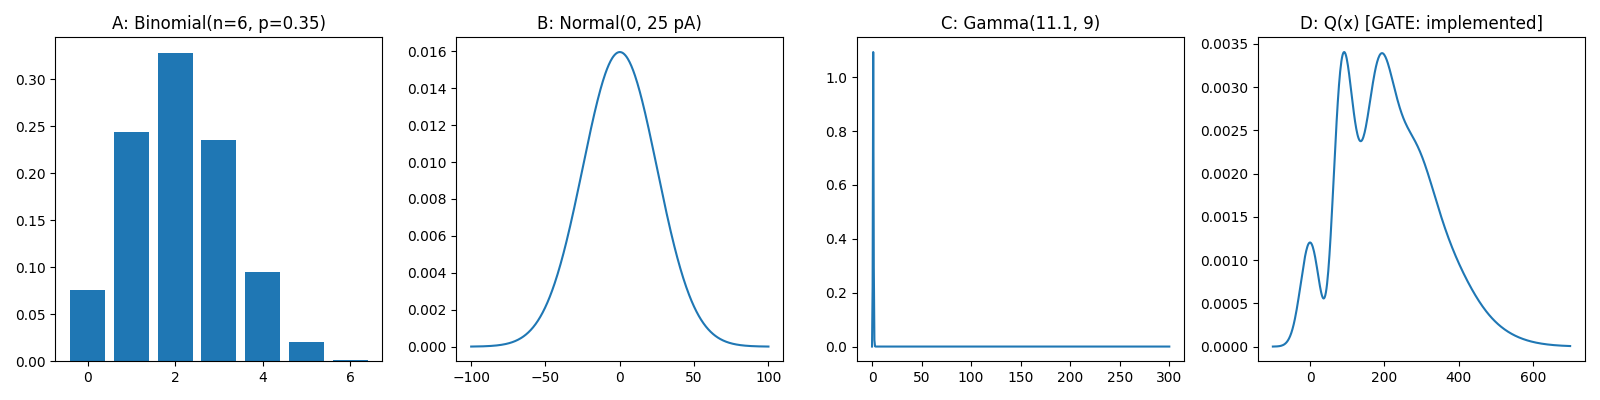
\includegraphics{figures/figure1_feasibility_gate.png}
\caption{Reproduction of the original Figure 1A-D. Panels A-C are the binomial, Gaussian, and gamma components. Panel D is the combined quantal likelihood \(Q\) and is multimodal with peaks near multiples of the 100 pA quantal size, as the original describes.}\label{fig:gate}
\end{figure}

\section{Beyond the original paper}

\subsection{Simulation-based calibration}
\label{sec:sbc}

SBC draws parameters from the prior, simulates data from the model, runs the inference, and records where each true value falls within its posterior. If the inference is calibrated, those ranks are uniform \supercite{talts2018}. The original paper did not run this check.

SBC needed one modeling choice the paper does not make. The paper treats each condition mean \(\mu_k\), and therefore \(q\), as a known input, so it never gives \(q\) a prior. Simulating data needs a true \(q\), so we added a log-uniform prior on \(q\) over \([10, 1000]\) pA as scaffolding for the test. It is labeled as such in the code and is not a claim about the paper's model. Baseline variance is fixed to the paper's value. Because BQA is a grid method, each rank is a probability integral transform (PIT) read from the grid marginal, and the discrete site count uses a jittered rank to avoid the spurious histogram structure plain ranks produce on discrete parameters\supercite{sailynoja2022}. All \(p\)-values below are per-parameter Kolmogorov-Smirnov tests against uniformity, uncorrected for multiple comparisons, as is usual for SBC diagnostics.

\paragraph{An error in our own rank statistic.}
Our first powered run reported the quantal-size intervals as badly miscalibrated and too narrow: a nominal 90\% interval covered 81 to 84\% of true values, with the whole shortfall in the upper tail. The cause was our PIT function, not BQA. It computed the rank as the mass below the true value plus half the mass of one cell, but \texttt{np.searchsorted} returns the cell \emph{above} the true value, so the whole cell below had already been counted and the half credit went to the wrong cell. The error is at most one cell's mass and never negative, so it pushed every rank upward. It mattered most where the posterior was narrow relative to the grid, which is why \(q\) and \(r\) failed while the discrete \(n\), ranked by a separate code path, did not.

Three checks confirm the diagnosis (Table~\ref{tab:pit}; \texttt{src/pit\_diagnostics.py}). Fed samples from a known lognormal on the same log-spaced axis, with no BQA involved, the old function returns non-uniform ranks (KS \(p = 0.0026\), 5.9\% above the 95th percentile against 4.7\% below) and the corrected one returns uniform ranks (\(p = 0.11\)). On identical posteriors the corrected transform moves the quantal-size result from failing to passing. And because \(q = \mu/(np)\) is decreasing in \(p\) at fixed \(\mu\) and \(n\), ranking the same posterior on the release-probability axis must give one minus the \(q\) rank; the old function instead gives a mirror-image failure in the lower tail, which is what an error in the transform predicts. The old function is kept in the code as \texttt{weighted\_cdf\_pit\_legacy} so the superseded numbers can be regenerated.

\begin{table}[!htb]
\centering
\caption{The same 200 single-condition posteriors, with the site count fixed to its true value, ranked by the old and the corrected PIT. Coverage is of a nominal 90\% central interval; the last two columns are the fractions of true values above the 95th and below the 5th posterior percentile, each 5\% if calibrated. From \texttt{results/calibration/pit\_diagnostics\_summary.csv}.}
\label{tab:pit}
\small
\begin{tabular}{@{}llrrrr@{}}
\toprule
route & PIT & KS \(p\) & coverage & above \(p_{95}\) & below \(p_{05}\) \\
\midrule
\(q\) axis, resolution 128 & old & \(1.2\times10^{-8}\) & 0.810 & 0.170 & 0.020 \\
\(q\) axis, resolution 128 & corrected & 0.107 & 0.935 & 0.045 & 0.020 \\
\(q\) axis, resolution 256 & old & \(2.0\times10^{-5}\) & 0.880 & 0.100 & 0.020 \\
\(q\) axis, resolution 256 & corrected & 0.082 & 0.915 & 0.060 & 0.025 \\
\(p\) axis, mapped to \(q\) & old & 0.004 & 0.855 & 0.035 & 0.110 \\
\(p\) axis, mapped to \(q\) & corrected & 0.037 & 0.920 & 0.055 & 0.025 \\
\bottomrule
\end{tabular}
\end{table}

We report this error because it is easy to make. A grid posterior has no samples to rank, so every grid-based SBC needs a hand-written PIT, and an error in it looks exactly like an overconfident posterior. Running the transform on a distribution with a known answer, as in the first check above, would have caught it before any BQA run.

\paragraph{Calibration of the reproduced method.}
With the corrected PIT, the reproduced method (product combination, 200 draws) gives unbiased point estimates (median \(\hat q/q_{\mathrm{true}} = 0.997\)) and calibrated total response \(r\) (KS \(p = 0.31\)), variability \(\gamma\) (\(p = 0.45\)) and site count \(n\) (\(p = 0.22\)). Quantal size fails the uniformity test (\(p = 0.007\)), but the rank histogram is domed, not skewed (Figure~\ref{fig:sbc}): too few true values land in either tail (2.5\% above the 95th percentile, 3.0\% below the 5th), and a nominal 90\% interval covers 94.5\%. The quantal-size interval is somewhat too wide. For a user, that means it can be read as a conservative bound.

\begin{figure}[!htb]
\centering
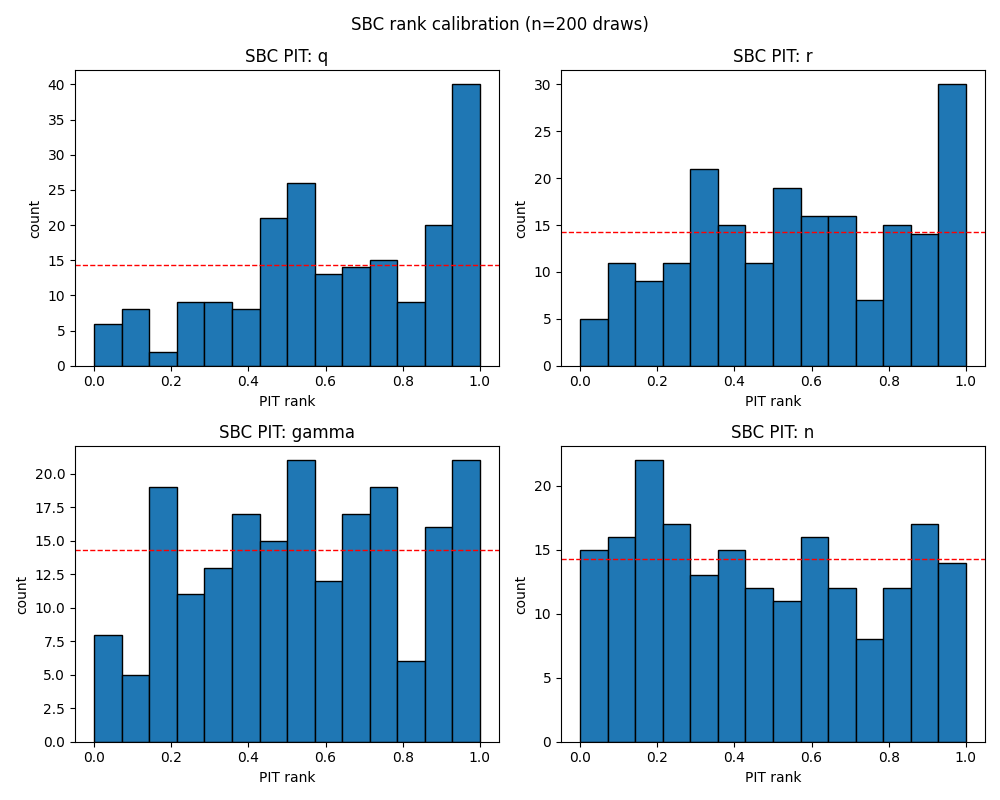
\includegraphics{figures/sbc_rank_histograms.png}
\caption{SBC rank (PIT) histograms for \(q\), \(r\), \(\gamma\), and \(n\), reproduced product method, 200 draws, and corrected PIT. The dashed line is the count expected under uniformity. The \(q\) histogram is domed, with thin tails: the interval is too wide, not too narrow. The other three are consistent with uniform.}
\label{fig:sbc}
\end{figure}

\paragraph{Where the extra width comes from.}
We removed the machinery one piece at a time, using single-condition runs (\(K = 1\)) so that no combination step is involved, and the exact prior implied by the SBC generator (\texttt{q\_prior="induced"}; at \(K = 1\) it gives the same posterior as the default \texttt{geometric} prior). Table~\ref{tab:nmarg} shows the result. With the site count fixed to its true value, quantal size is calibrated (\(p = 0.107\), 93.5\% coverage). Allowing three or five candidate values of \(n\) centered on the truth makes it fail, and coverage rises to 95 and 96\% while the upper tail shrinks from 4.5 to 2\%. Doubling the grid resolution does not change this, so it is not a discretisation effect. The spread of the ranks falls below the uniform value as more candidates are added (Figure~\ref{fig:nmarg}), which is the signature of a posterior that is too wide. The sum over \(n\) is therefore the source of the conservative quantal-size interval. The log-uniform prior that matches the generator's own \(q\) draw behaves the same way (\(p = 0.020\)).

\begin{table}[!htb]
\centering
\caption{Quantal-size SBC at \(K = 1\) as the candidate set for \(n\) widens, 200 draws each, corrected PIT. The full set is \(\{4, \dots, 8\}\), the setting used in the other single-condition runs. From \texttt{sbc\_n\_marginalisation\_summary.csv}.}
\label{tab:nmarg}
\small
\begin{tabular}{@{}lrrrrr@{}}
\toprule
candidates for \(n\) & KS \(p\) & coverage & above \(p_{95}\) & below \(p_{05}\) & median \(\hat q/q\) \\
\midrule
true \(n\) only & 0.107 & 0.935 & 0.045 & 0.020 & 0.995 \\
true \(n \pm 1\) (3 values) & 0.003 & 0.950 & 0.030 & 0.020 & 0.999 \\
true \(n \pm 2\) (5 values) & \textless0.001 & 0.960 & 0.020 & 0.020 & 0.992 \\
true \(n \pm 2\), resolution 256 & 0.005 & 0.945 & 0.035 & 0.020 & 0.998 \\
full set \(\{4, \dots, 8\}\) & 0.004 & 0.945 & 0.035 & 0.020 & 0.998 \\
\bottomrule
\end{tabular}
\end{table}

\begin{figure}[!htb]
\centering
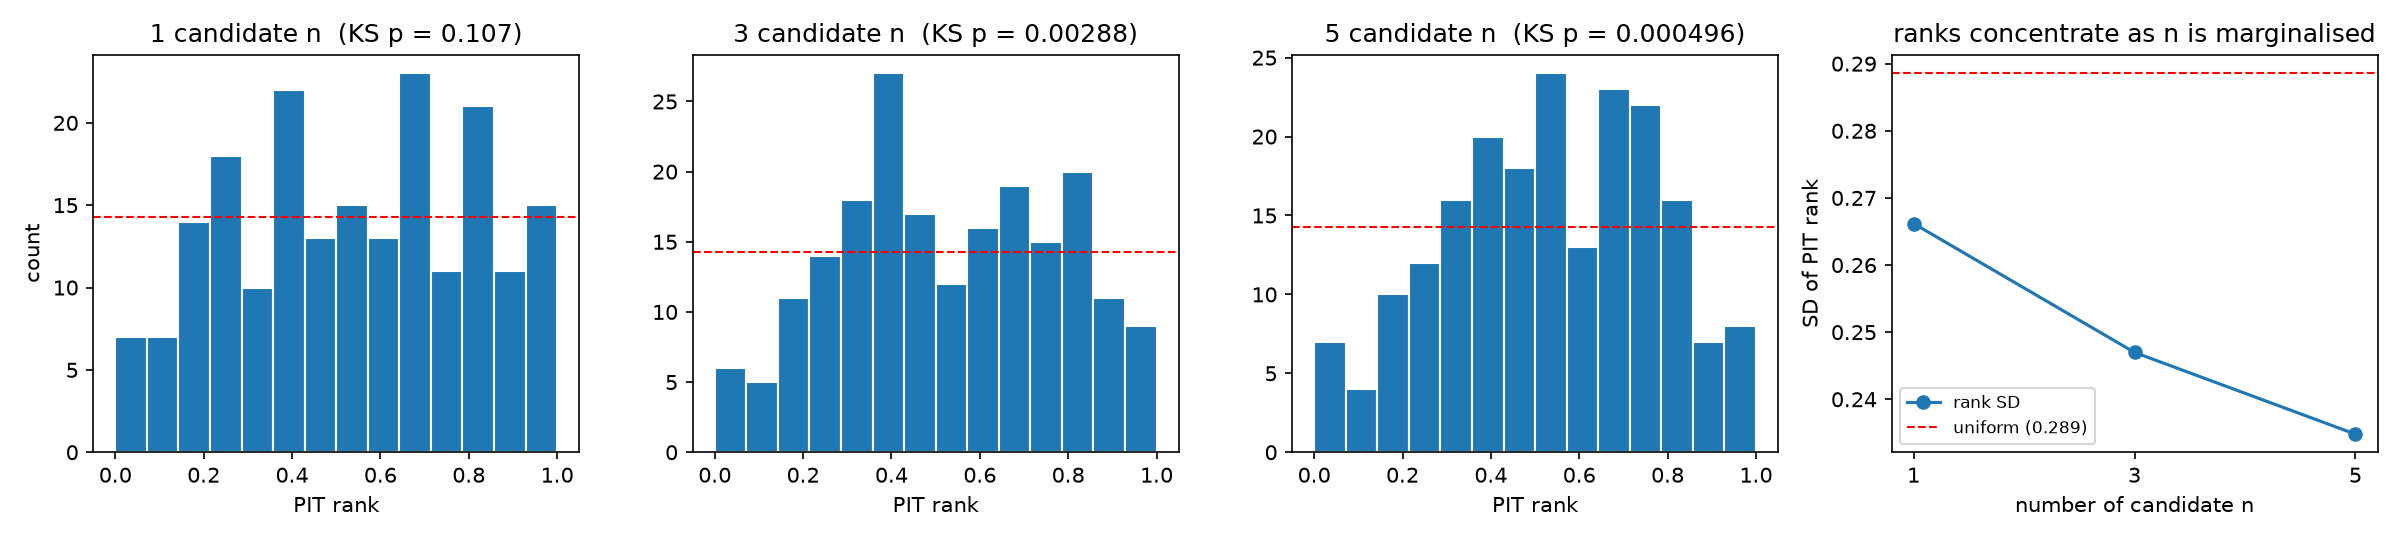
\includegraphics{figures/n_marginalisation_sweep.png}
\caption{Quantal-size PIT histograms at \(K = 1\) with 1, 3, and 5 candidate values of \(n\), and (right) the standard deviation of the ranks against the number of candidates. The dashed line in the right panel is the value for uniform ranks (0.289). Ranks concentrate in the middle as \(n\) is marginalized, so the posterior is wider than the spread of the true values.}
\label{fig:nmarg}
\end{figure}

The SBC harness passes the true condition mean \(\mu = npq\) to the inference, while real use passes the sample mean of the same amplitudes that enter the likelihood. We checked whether this matters by rerunning the fixed-\(n\) configuration with the sample mean on the same draws. Coverage drops from 93.5 to 88.9\% (KS \(p = 0.027\), 199 usable draws), so using the data twice makes the interval slightly too narrow. The effect is small and runs opposite to the \(n\)-marginalization effect.

\paragraph{Combination rules and the joint grid.}
The paper combines conditions by normalizing each condition's grid, moving it onto the shared \(q\)-axis, and multiplying. This carries the prior once per condition, so we expected it to over-sharpen the posterior. We built three alternatives: combining the raw log-likelihoods once (\texttt{combine="loglik"}), a bin-width correction (\texttt{combine="density"}), and a single joint grid (\texttt{combine="joint"}). The joint grid evaluates the whole likelihood once over the shared parameters: for each candidate \(n\) the grid runs over \((q, v)\), each condition's release probability is set to \(p_k = \mu_k / (n q)\), the Eq.~8 log-likelihoods are summed across conditions, and the prior on \(q\) is added once. There is no per-condition normalization and no mass transport. The joint posterior normalizes to one, and on single-condition data it gives the same point estimate as the product rule; both are asserted in the test suite.

The data do not support the over-sharpening hypothesis (Table~\ref{tab:scaling}). Posterior width falls as conditions are added under every rule, including the joint grid, which has no double-counted prior. The product rule is never narrower than the joint grid; it is slightly wider at every condition count, because the nearest-bin transport spreads mass. Only the log-likelihood rule is consistently wider. Most of the narrowing is therefore the information in the added conditions, not an artifact of the combination step. In this harness no rule is calibrated at every condition count.

\begin{table}[!htb]
\centering
\caption{Quantal-size SBC as conditions are added, for four combination rules (\texttt{src/conditions\_scaling.py}, 120 draws, independent seed per draw, corrected PIT). SD is the mean posterior standard deviation of \(q\) in pA.}
\label{tab:scaling}
\small
\setlength{\tabcolsep}{5pt}
\begin{tabular}{@{}lrrrrrrrr@{}}
\toprule
& \multicolumn{2}{c}{product} & \multicolumn{2}{c}{log-lik}
& \multicolumn{2}{c}{density} & \multicolumn{2}{c}{joint} \\
\cmidrule(lr){2-3}\cmidrule(lr){4-5}\cmidrule(lr){6-7}\cmidrule(lr){8-9}
conditions & KS \(p\) & SD & KS \(p\) & SD & KS \(p\) & SD & KS \(p\) & SD \\
\midrule
1 & \textless0.001 & 33.8 & 0.019 & 38.2 & \textless0.001 & 33.8 & 0.041 & 28.8 \\
2 & 0.007 & 16.2 & \textless0.001 & 24.5 & 0.017 & 14.8 & 0.004 & 13.8 \\
3 & \textless0.001 & 11.1 & 0.034 & 17.0 & \textless0.001 & 10.5 & \textless0.001 & 10.5 \\
\bottomrule
\end{tabular}
\end{table}

The paper never places a prior on the derived shared \(q\), so the joint grid needs one. Table~\ref{tab:qprior} lists the four options we offer. Table~\ref{tab:priors} compares the product rule with the joint grid under three of them in the full 200-draw, two-condition SBC. Every variant keeps the point estimate unbiased, and every variant shows the same conservative quantal-size interval (92.5 to 94.5\% coverage). The joint grid gives no calibration gain over the product rule, and under the log-uniform prior it makes \(r\) and \(n\) worse. We keep the product rule as the default, since it is the method as reproduced from the paper, and ship the joint grid as a tested option.

\begin{table}[!htb]
\centering
\caption{Shared-\(q\) priors offered by the joint grid. \texttt{geometric} is the default.}
\label{tab:qprior}
\begin{tabular}{@{}l>{\raggedright\arraybackslash}p{0.62\linewidth}@{}}
\toprule
option & construction \\
\midrule
\texttt{geometric} & geometric mean of the \(K\) induced arcsine densities \\
\texttt{induced} & change-of-variables prior implied by the SBC generator, with the \((nq)^{-K}\) Jacobian \\
\texttt{reference} & first condition only \\
\texttt{flat} & log-uniform, matching the generator's own \(q\) draw \\
\bottomrule
\end{tabular}
\end{table}

\begin{table}[!htb]
\centering
\caption{Two-condition SBC, 200 draws, corrected PIT: per-parameter KS \(p\)-values (\(p > 0.05\) is consistent with calibration), 90\% coverage of \(q\), and the median ratio of estimate to truth. The last row repeats the log-uniform joint run at grid resolution 256. From \texttt{sbc\_report*.csv} and \texttt{sbc\_results*.csv}.}
\label{tab:priors}
\small
\begin{tabular}{@{}lrrrrrr@{}}
\toprule
method & \(q\) & \(r\) & \(\gamma\) & \(n\) & \(q\) coverage & median \(\hat q/q\) \\
\midrule
product (default) & 0.007 & 0.308 & 0.448 & 0.224 & 0.945 & 0.997 \\
joint, geometric & 0.004 & 0.009 & 0.360 & 0.226 & 0.945 & 0.996 \\
joint, induced & 0.001 & 0.206 & 0.117 & 0.315 & 0.945 & 0.996 \\
joint, flat & 0.008 & \textless0.001 & 0.588 & 0.021 & 0.935 & 0.997 \\
joint, flat, resolution 256 & 0.032 & 0.069 & 0.047 & 0.029 & 0.925 & 0.998 \\
\bottomrule
\end{tabular}
\end{table}

\begin{figure}[!htb]
\centering
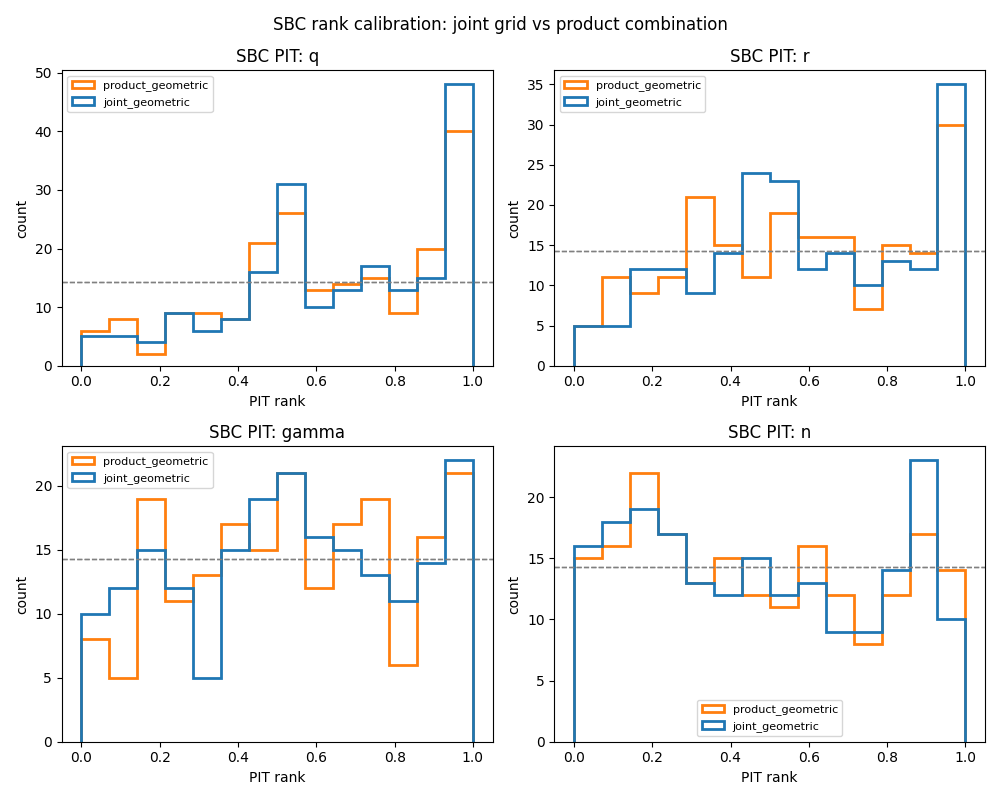
\includegraphics{figures/sbc_joint_vs_product.png}
\caption{SBC rank histograms, joint grid (blue) against the product rule (orange), on identical draws. Both give the same domed \(q\) histogram; neither is clearly better on the other three parameters.}\label{fig:joint}
\end{figure}

\subsection{Identifiability map}
\label{sec:ident}

To see where BQA resolves its parameters we fixed \(p_1 = 0.1\), swept the contrast \(\Delta P\) from 0.05 to 0.80 in steps of 0.01 with \(p_2 = p_1 + \Delta P\), and ran a full inference at each of the 76 points on data from the model's own likelihood. The 95\% credible-interval width of the \(q\) and \(n\) marginals measures identifiability: a wide interval means the parameter is poorly pinned down. Table~\ref{tab:ident} summarises the sweep.

\begin{table}[!htb]
\centering
\caption{Identifiability across the \(\Delta P\) sweep (76 inferences, true \(q = 100\) pA, true \(n = 6\), six candidate values for \(n\)).}
\label{tab:ident}
\begin{tabular}{@{}lrr@{}}
\toprule
& quantal size \(q\) & site count \(n\) \\
\midrule
mean point estimate & 98.7 pA & scatter 4.5 to 8.3 \\
range of point estimates & 81 to 119 pA & \\
mean 95\% interval width & 34.9 pA & 4.3 candidates \\
range of 95\% interval width & 11.8 to 57.4 pA & never below 2 \\
\bottomrule
\end{tabular}
\end{table}

Quantal size is the better-resolved parameter. Its interval width shows no clean trend with \(\Delta P\) since the scatter from point to point is as large as any trend (Figure~\ref{fig:ident}). The site count is weakly resolved from two conditions at these sample sizes, expected when \(n\) and \(p\) trade off and two release probabilities carry little information to separate them. That weak resolution is also what widens the quantal-size interval in SBC: uncertainty about \(n\) passes into \(q\) through \(q = \mu/(np)\).

\begin{figure}[!htb]
\centering
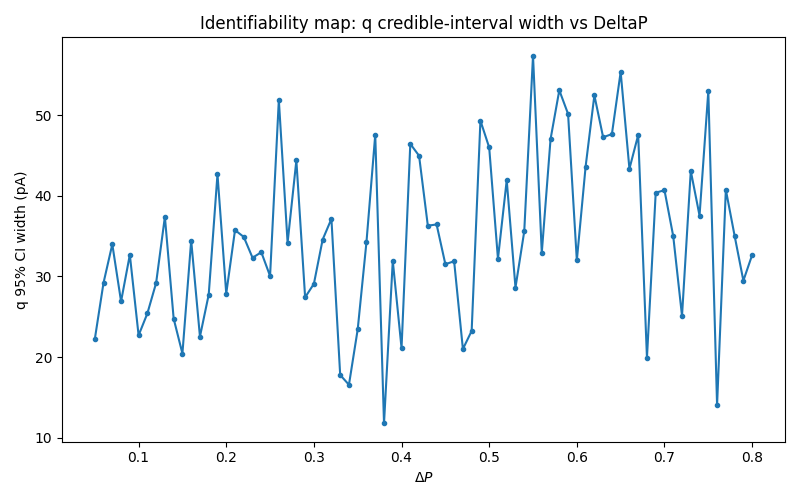
\includegraphics{figures/identifiability_map.png}
\caption{Identifiability map. 95\% credible-interval width of the \(q\) marginal against the release-probability contrast \(\Delta P\), one BQA inference per point. The width stays bounded and scattered instead of shrinking smoothly as the conditions separate, and the quantal-size estimate stays within 20\% of the truth across the sweep.}
\label{fig:ident}
\end{figure}

\subsection{Comparison with MPFA}
\label{sec:mpfa}

The original paper positions BQA against MPFA. We did not transcribe the MPFA estimator of \citet{silver2003}, but instead we implemented the general variance-mean relationship as a baseline. Across conditions that differ only in release probability, the mean evoked response is \(I = nPq\) and the evoked variance follows the parabola \(\sigma^2 = q(1+v^2)I - I^2/n\). The initial slope gives an apparent quantal size and the curvature gives the site count. Without an independent estimate of the variability, the \((1+v^2)\) factor makes the slope overestimate \(q\) by about 9\% at \(v = 0.3\).

We simulated seven release-probability conditions from the Gaussian model at the paper's constants and ran both estimators on the same data (Table~\ref{tab:mpfa}, Figure~\ref{fig:mpfa}). BQA gets close on quantal size and estimates the variability itself. MPFA's raw slope is biased upward by exactly the term BQA infers. MPFA's site count is closer to the truth on this draw. This is a single simulated data set, so we do not read anything into the size of either margin; the systematic difference is the \((1+v^2)\) inflation.

\begin{table}[!htb]
\centering
\caption{BQA against MPFA on identical data from seven release-probability conditions. The variability-corrected MPFA row needs the true \(v\) supplied from outside the method.}
\label{tab:mpfa}
\begin{tabular}{@{}lrrr@{}}
\toprule
method & \(q\) (pA) & \(n\) & \(v\) \\
\midrule
truth & 100 & 6 & 0.30 \\
MPFA, apparent & 103 & 6.2 & needs external estimate \\
MPFA, variability-corrected & 94.6 & 6.2 & needs external estimate \\
BQA & 98.3 & 5.6 & 0.35 (estimated) \\
\bottomrule
\end{tabular}
\end{table}

\begin{figure}[!htb]
\centering
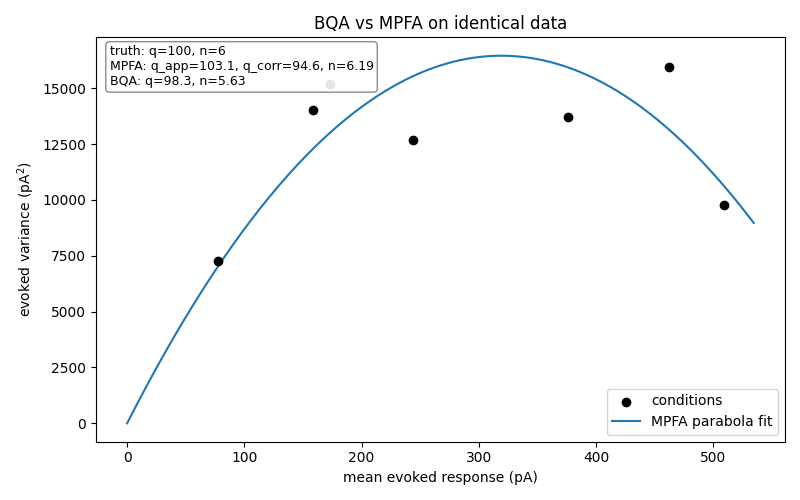
\includegraphics{figures/mpfa_vs_bqa.png}
\caption{BQA against MPFA on identical data. Points are the per-condition mean and evoked variance across seven release-probability conditions; the curve is the fitted variance-mean parabola. The inset lists both methods' quantal-size and site-count estimates against the truth.}\label{fig:mpfa}
\end{figure}

\subsection{Robustness to Gaussian-versus-gamma mismatch}
\label{sec:mismatch}

The paper reports that BQA estimates quantal size accurately even when the true per-quantum variability is Gaussian rather than the gamma its likelihood assumes. We tested this by generating two-condition data with the Gaussian simulator and fitting it with the gamma likelihood. The recovered quantal size was 95.6 pA against a true 100 pA, and the site count 5.9 against a true 6 (Figure~\ref{fig:mismatch}). At the paper's signal-to-noise the mismatch costs a few percent. Section~\ref{sec:lowsnr} shows that this tolerance does not hold at weaker signal.

\begin{figure}[!htb]
\centering
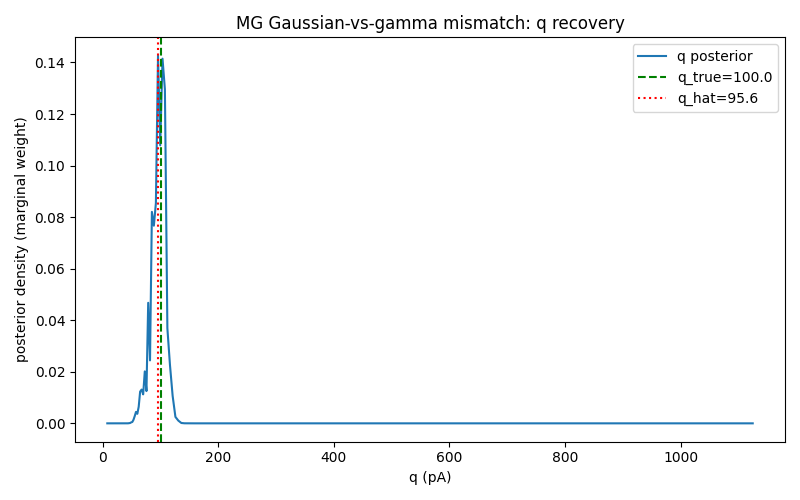
\includegraphics{figures/mg_detectability.png}
\caption{Gamma-likelihood BQA fitted to Gaussian-simulated data: the \(q\) marginal posterior, with the true value (100 pA) and the estimate (95.6 pA) marked. The posterior sits near the truth despite the mismatch.}\label{fig:mismatch}
\end{figure}

\subsection{Low signal-to-noise}
\label{sec:lowsnr}

We then ran a harder scenario, loosely modelled on myasthenia gravis, where receptor loss lowers the quantal size while the site count stays high: \(q = 30\) pA, \(n = 12\), baseline SD 25 pA, 100 observations per condition, \(p_1 = 0.15\), \(p_2 = 0.45\), and candidates \(n \in \{4, \dots, 20\}\). Baseline noise is 83\% of the quantal size here, against 25\% in the paper's scenario.

Both parameters come back badly biased (Table~\ref{tab:lowsnr}, first row). Two design details matter for reading this correctly. The candidate set has to be wide: on the narrower \(\{8, \dots, 16\}\) set we used first, several seeds put \(\hat n\) within one bin of the lower edge, their posterior mass is clipped, and the ensemble mean is pulled toward the truth. And one seed is not enough: on that narrow set, seed 42 alone returns \(\hat n = 12.3\), which would have looked like an accurate recovery.

\begin{table}[!htb]
\centering
\caption{Low signal-to-noise ensemble, twelve seeds per row, true \(q = 30\) pA and \(n = 12\), candidates \(n \in \{4,\dots,20\}\). The resolution rows report the mean absolute quantal-size error instead of the estimate. From \texttt{results/identifiability/low\_snr\_seed\_ensemble.csv} (\texttt{src/low\_snr\_seeds.py}).}
\label{tab:lowsnr}
\small
\setlength{\tabcolsep}{4pt}
\begin{tabular}{@{}llrr@{}}
\toprule
generator & configuration & \(\hat q\) (pA) & \(\hat n\) \\
\midrule
Gaussian & resolution 128 (default) & \(38.2 \pm 4.5\) \; (\(+27\%\)) & \(7.9 \pm 2.4\) \; (\(-34\%\)) \\
Gaussian & resolution 64, mean abs.\ error & 8.39 & 7.88 \\
Gaussian & resolution 128, mean abs.\ error & 8.23 & 7.87 \\
Gaussian & resolution 256, mean abs.\ error & 8.43 & 7.86 \\
matched (Eq.~8) & resolution 128 & \(29.2 \pm 2.0\) \; (\(-2.8\%\)) & \(13.3 \pm 3.0\) \\
\bottomrule
\end{tabular}
\end{table}

Grid resolution is not the cause: rerunning the same twelve seeds at resolutions 64, 128, and 256 leaves the quantal-size error and the site-count estimate essentially unchanged (Table~\ref{tab:lowsnr}). Weak signal alone is not the cause either. The data here are Gaussian while the likelihood is gamma, so the scenario mixes low signal-to-noise with model misspecification. Rerunning it with the matched generator (\texttt{simulate\_from\_q\_model}) separates the two: quantal size becomes essentially unbiased, and the site count comes back to within one standard deviation of 12. The bias is misspecification made worse by weak signal, and the tolerance shown in Section~\ref{sec:mismatch} at 25\% relative noise does not extend to 83\%.

The matched arm shows the same pattern as the rest of the paper: quantal size is recovered tightly and the site count is noisy (SD 3.0 on a 17-value candidate set). Estimates are read off a log-spaced grid at resolution 128, so identical \(\hat q\) values recur across seeds and the quoted standard deviations are lower bounds.

\section{Discussion}

The likelihood and the grid inference reproduce. SBC, which the original paper did not run, supports the method because point estimates are unbiased, the total-response, variability, and site-count marginals are calibrated, and the quantal-size interval errs on the safe side, covering about 94\% of true values at a nominal 90\%. We traced that extra width to the sum over candidate site counts. It is consistent with the identifiability sweep, where \(n\) is weakly resolved from two conditions and its uncertainty passes into \(q\).

The main risk for a user is not the calibration but the model assumptions. At the paper's signal-to-noise, Gaussian per-quantum variability costs a few percent. At 83\% relative noise it produces a 27\% quantal-size bias and a 34\% site-count bias, and only the matched-generator control recovers either. We did not find evidence that the paper's combine-then-multiply step over-sharpens the posterior. The joint grid, which avoids it, is no better calibrated and is slightly narrower.

The first version of this analysis reached the opposite conclusion about calibration because of an error in our own PIT function. We describe it in Section~\ref{sec:sbc} because the failure can be easily made. Grid posteriors need a hand-written rank transform, and an off-by-one-cell error in that transform produces a clean, one-sided, resolution-stable miscalibration that looks like a real property of the method. Testing the transform on a distribution with a known answer catches it.

Several limitations remain. Grid-cell resampling uses nearest-bin histogram assignment by default, which slightly widens the product-rule posterior. The per-condition likelihood is a vectorized re-implementation of Eq.~8 for speed, and a test asserts that it agrees with the reference cell for cell. The heterogeneous-release extension (Eqs.~A12-A13) is implemented and tested on its own but is not wired into the main pipeline. Original Figures 4, 7, and 8 were not reproduced, and Figure 2 was reproduced as one inference per \(\Delta P\) instead of 100-simulation histograms. The MPFA comparison uses a textbook variance-mean parabola instead of the full estimator of \citet{silver2003} and a single simulated data set, so it is a baseline, not a reproduction of that method.

\subsection{Reproducibility}

The test suite (36 tests) passes, and \texttt{bash\ reproduce.sh} regenerates every figure and CSV in this article from a fresh clone in about 40 minutes on a laptop. Dependency versions are pinned in \texttt{requirements.txt} (Python 3.13). Each analysis writes its numbers to a committed CSV, so the values quoted here come from files rather than figure pixels. The resolution sweep and the low signal-to-noise test both use an explicit twelve-seed ensemble, so their rows differ in grid resolution and seed together.

\section{Conclusion}

BQA, rebuilt from the paper alone, behaves as described. Its likelihood reproduces the original's central figure, and its grid inference recovers parameters from model-generated data with unbiased point estimates.

Its credible intervals can be used as stated for total response, variability, and site count. The quantal-size interval is conservative, covering about 94\% at a nominal 90\%, because the sum over candidate site counts widens it. The site count itself is poorly resolved from two release-probability conditions.

Both conclusions hold only while the quantal amplitude is well above the baseline noise and the per-quantum variability is close to gamma. At 83\% relative noise with Gaussian-generated data, quantal size runs 27\% high and the site count 34\% low. The noise ratio is the first thing to check before trusting either output.

\section*{Code availability}

All code, tests, and the CSV files behind every number in this article are at \url{https://github.com/AngadKumar16/ReScience-C}. \texttt{bash reproduce.sh} runs the test suite and regenerates every figure and CSV.

\section*{AI Disclosure}

The authors used ChatGPT and TexGPT to edit the manuscript and help maintain a formal tone across this work. The authors checked and verified all work done by these AI. 

\hypersetup{linkcolor=black,urlcolor=darkgray}
\renewcommand\emph[1]{{\bfseries #1}}
\setlength\bibitemsep{0pt}
\printbibliography

\end{document}